\documentclass[../main.tex]{subfiles}

\begin{document}

\begin{example}[Gysin sequence]
Suppose $F\to E\to B$ be a filtration, with $F=S^k$, then $E^2_{p,q}=H_p(B;H_q(F))=H_p(B)\otimes H_q(F)$ by universal coefficient theorem, since $H_q(F)=\begin{cases}
\mathbb Z, &q=0,k \\
0, &\text{Otherwise}
\end{cases}$, we have the second page
\begin{center}
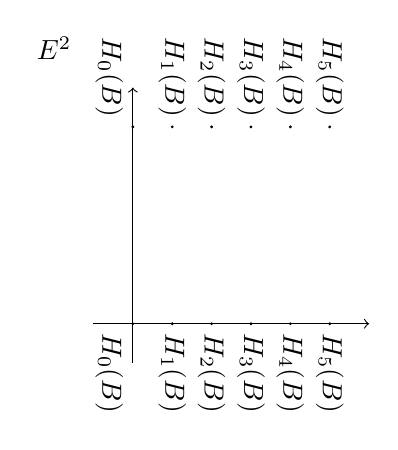
\begin{tikzpicture}[scale=0.5]
\draw[->](-1,0)--(6,0);
\draw[->](0,-1)--(0,6);
\foreach \x in {0,5}
{
\foreach \y in {0,1,...,5}
{
\filldraw (\y,\x) circle (0.02);
}
}
\node at (-2,7) {$E^2$};
\foreach \z in {1,...,5}
{
\node[rotate=-90, right] at (\z,0) {$H_{\z}(B)$};
\node[rotate=-90, left] at (\z,5) {$H_{\z}(B)$};
}
\node[rotate=-90, below right] at (0,0) {$H_{0}(B)$};
\node[rotate=-90, below left] at (0,5) {$H_{0}(B)$};
\end{tikzpicture}
\end{center}
The only non trivial differential appears on page $k+1$, thus we have $E^2=E^3=\cdots=E^{k+1}$, $E^{k+2}=E^{k+3}=\cdots=E^\infty$, on page $k+1$, we have $\partial^{k+1}:E^{k+1}_{r,0}\to E^{k+1}_{r-k-1,k}$, thus $\ker\partial^{k+1}=E^{k+2}_{r,0}=E^{\infty}_{r,0}$, $\mathrm{coker}\partial^{k+1}=E^{k+2}_{r-k-1,k}=E^{\infty}_{r-k-1,k}$
\begin{center}
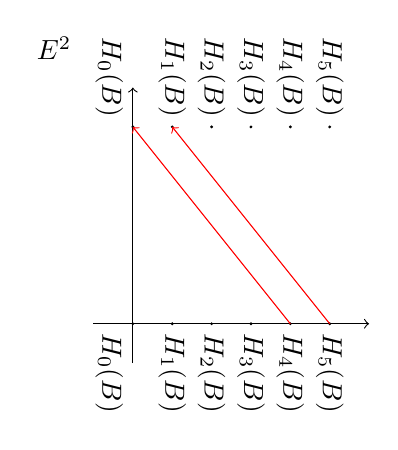
\begin{tikzpicture}[scale=0.5]
\draw[->](-1,0)--(6,0);
\draw[->](0,-1)--(0,6);
\foreach \x in {0,5}
{
\foreach \y in {0,1,...,5}
{
\filldraw (\y,\x) circle (0.02);
}
}
\node at (-2,7) {$E^2$};
\foreach \z in {1,...,5}
{
\node[rotate=-90, right] at (\z,0) {$H_{\z}(B)$};
\node[rotate=-90, left] at (\z,5) {$H_{\z}(B)$};
}
\node[rotate=-90, below right] at (0,0) {$H_{0}(B)$};
\node[rotate=-90, below left] at (0,5) {$H_{0}(B)$};
\draw[red,->] (4,0)--(0,5);
\draw[red,->] (5,0)--(1,5);
\end{tikzpicture}
\end{center}
Therefore we get an exact sequence
\[0\to E^\infty_{r,0}\to H_r(B)\to H_{r-k-1}(B)\to E^{\infty}_{r-k-1,k}\to0\]
Since $H_n(E)=E^\infty_{n-k,k}\oplus E^\infty_{n,0}$, there is also an exact sequence
\[0\to E^\infty_{n-k,k}\to H_n(E)\to E^\infty_{n,0}\to0\]
Put them together, we get the \textbf{Gysin sequence}\index{Gysin sequence}
\[\cdots\to H_n(E)\to H_{n}(B)\to H_{n-k-1}(B)\to H_{n-1}(E)\to\cdots\]
\end{example}

\begin{theorem}
Suppose $C_*$ is filtered chain complex, then there is a spectral sequence $E^1_{p,q}=H_{p+q}(F_pC/F_{p-1}C)\Rightarrow H_{p+q}(C)$ with differential $\partial^1:H_{p+q}(F_pC/F_{p-1}C)\to H_{p+q-1}(F_{p-1}C/F_{p-2}C)$ induced by the composition of boundary map and quotient map 
$H_{p+q}(F_pC/F_{p-1}C)\to H_{p+q-1}(F_{p-1}C)\to H_{p+q-1}(F_{p-1}C/F_{p-2}C)$
\end{theorem}

\begin{remark}
Suppose the filtration is in the first quadrant, we can view $Z^r_{p,q}$ as
\[\left\{c\in F_pC_{p+q}\middle|\partial c\in F_{p-r}C_{p+q-1}\right\}+F_{p-1}C_{p+q}\]
$B^r_{p,q}$ as
\[\partial F_{p+r-1}C_{p+q+1}+F_{p-1}C_{p+q}\]
$E^r_{p,q}$ as
\[\frac{\left\{c\in F_pC_{p+q}\middle|\partial c\in F_{p-r}C_{p+q-1}\right\}+F_{p-1}C_{p+q}}{\partial F_{p+r-1}C_{p+q+1}+F_{p-1}C_{p+q}}\]
Then $Z^0_{p,q}=F_pC_{p,q}$, $B^0_{p,q}=F_{p-1}C_{p+q}$, $E^0_{p,q}=F_pC_{p+q}/F_{p-1}C_{p+q}$, $E^1_{p,q}=H_{p+q}(F_pC_*/F_{p-1}C_*)$ \par
$Z^\infty_{p,q}=\left\{c\in F_pC_{p+q}\middle|\partial c=0\right\}+F_{p-1}C_{p+q}$, $B^\infty_{p,q}=\partial C_{p+q+1}+F_{p-1}C_{p+q}$, $E^\infty_{p,q}=\dfrac{Z_{p+q}(F_pC_*)+F_{p-1}C_{p+q}}{B_{p+q}(C_*)+F_{p-1}C_{p+q}}=\dfrac{F_pH_{p+q}(C)}{F_{p-1}H_{p+q}(C)}=\dfrac{\mathrm{im}(H_{p+q}(F_pC)\to H_{p+q}(C))}{\mathrm{im}(H_{p+q}(F_{p-1}C)\to H_{p+q}(C))}$
\end{remark}

\begin{example}
Let $X$ be a CW complex, consider $C_*=C_*^{\mathrm{sing}}(X)$, $F_pC_*=C_*^{\mathrm{sing}}(X^p)$, $E^1_{p,q}=H_{p+q}(X^p,X^{p-1})=\begin{cases}
C^\mathrm{cell}_p(X), &q=0 \\
0, & \text{Otherwise}
\end{cases}$, $\partial^1$ is just the cellular boundary map, thus $E^2_{p,0}=E^\infty_{p,0}=H_p^{\mathrm{cell}}(X)\cong H^\mathrm{sing}_p(X)$
\end{example}

\begin{example}
Suppose $A\subseteq X$ is a subspace, consider $0\subseteq C_*(A)\subseteq C_*(X)$, $E^1_{1,q}=H_{q+1}(X,A)$, $E^1_{0,q}=H_q(A)$ with $\partial^1:H_{q+1}(X,A)\to H_q(A)$ induced by the boundary map, then we have exact sequences
\[0\to E^\infty_{1,q}\to H_{q+1}(X,A)\to H_q(A)\to E^\infty_{0,q}\to0\]
\[0\to E^\infty_{0,n}\to H_n(X)\to E^\infty_{1,n-1}\to0\]
Which give us the long exact sequence for $(X,A)$
\end{example}

\begin{definition}
A \textbf{double complex}\index{Double complex} $C_{*,*}$ is $\mathbb Z$-bigraded with two differentials $\partial':C_{p,q}\to C_{p-1,q}$, $\partial':C_{p,q}\to C_{p,q-1}$ such that $(\partial')^2=(\partial'')^2=0$ and $\partial'\partial''+\partial''\partial'=0$($\partial',\partial''$ anticommutes) \par
Define the \textbf{total chain complex}\index{Total chain complex} $Tot_n:=\displaystyle\bigoplus_{p+q=n}C_{p,q}$, $\partial=\partial'+\partial''$
\end{definition}

\begin{example}
Suppose $C_*,D_*$ are chain complexes, $C_*\otimes D_*$ is defined to be the total complex of the double complex $C_{p,q}:= C_p\otimes D_q$, $\partial':=\partial^C\otimes1$, $\partial'':=(-1)^p1\otimes\partial^D$
\end{example}

\end{document}